\documentclass[11pt,a4paper]{article}

\usepackage[spanish,es-nodecimaldot]{babel}
\usepackage[utf8]{inputenc}
\usepackage[T1]{fontenc}
\usepackage{lmodern}
\usepackage[margin=2.5cm]{geometry}
\usepackage{graphicx}
\usepackage{booktabs}
\usepackage{array}
\usepackage{hyperref}
\usepackage{xcolor}
\usepackage{float}
\usepackage{enumitem}
\usepackage{tikz}
\usepackage{fancyhdr}
\usepackage{ragged2e}
\usepackage{amsmath}

\hypersetup{colorlinks=true, linkcolor=blue, urlcolor=blue}
\pagestyle{fancy}
\fancyhf{}
\fancyfoot[R]{\thepage}
\renewcommand{\headrulewidth}{0pt}
\renewcommand{\footrulewidth}{0pt}

\title{\textbf{Implementación de una red neuronal desde cero}\\
\large Informe técnico}
\author{Gianfranco Giannoni\\
\small Herramientas para Ciencias de Datos (INFB6052)\\
\small Docente: Michael Miranda\\
\small Universidad Tecnológica Metropolitana}
\date{10 de noviembre de 2026}

\begin{document}

\begin{titlepage}

\begin{tikzpicture}[remember picture,overlay]
\node[
    anchor=north west,
    xshift=1.5cm,
    yshift=-1.2cm
] at (current page.north west) {
    
\includegraphics[width=2.4cm]{logo_utem.png}
};
\end{tikzpicture}

\vspace*{3cm}

\begin{center}

{\LARGE\bfseries Implementación de una red neuronal desde cero\par}

\vspace{0.4cm}

{\large Informe técnico\par}

\vspace{1.5cm}

{\large Gianfranco Giannoni\par}

\vspace{0.2cm}

{\normalsize Herramientas para Ciencias de Datos (INFB6052)\par}

{\normalsize Docente: Michael Miranda\par}

{\normalsize Universidad Tecnológica Metropolitana\par}

\end{center}

\vfill

\begin{center}
{\normalsize 10 de noviembre de 2026\par}
\end{center}

\end{titlepage}

\tableofcontents
\thispagestyle{empty}
\clearpage
\justifying

\section{Resumen}
Este informe describe la implementación de una red neuronal artificial desde cero utilizando Python y NumPy, sin recurrir a frameworks de aprendizaje profundo. El modelo corresponde a un perceptrón multicapa con dos entradas, una capa oculta de cuatro neuronas y una salida. Se entrenó para resolver el problema XOR mediante propagación hacia adelante, cálculo de pérdida, retropropagación del error y descenso del gradiente. En los cuatro ejemplos utilizados durante el entrenamiento, el modelo obtuvo las cuatro clases esperadas.

\section{Objetivos}
\begin{itemize}[leftmargin=*]
    \item Implementar los componentes básicos de una red neuronal utilizando operaciones matriciales.
    \item Aplicar funciones de activación y una función de pérdida apropiada para clasificación binaria.
    \item Entrenar la red mediante retropropagación y descenso del gradiente.
    \item Evaluar el comportamiento del modelo en el problema lógico XOR.
\end{itemize}

\section{Problema y datos}
Se utilizó el problema XOR, cuya salida es 1 cuando las dos entradas son distintas y 0 cuando son iguales. El conjunto contiene cuatro combinaciones:

\begin{table}[H]
\centering
\begin{tabular}{cc|c}
\toprule
$x_1$ & $x_2$ & $y$\\
\midrule
0 & 0 & 0\\
0 & 1 & 1\\
1 & 0 & 1\\
1 & 1 & 0\\
\bottomrule
\end{tabular}
\caption{Tabla de verdad del problema XOR.}
\end{table}

Este problema es útil como demostración porque no es linealmente separable: una única neurona sin capa oculta no puede representar correctamente sus cuatro casos.

\section{Metodología}
\subsection{Arquitectura}
La red implementada tiene arquitectura 2--4--1: dos variables de entrada, cuatro neuronas en la capa oculta y una neurona de salida. La capa oculta utiliza ReLU y la salida utiliza Sigmoid para producir una probabilidad entre 0 y 1.

\[
Z_1=XW_1+b_1,\qquad A_1=\operatorname{ReLU}(Z_1)
\]
\[
Z_2=A_1W_2+b_2,\qquad \hat{Y}=\sigma(Z_2)
\]

\subsection{Función de pérdida}
Se utiliza Binary Cross-Entropy (BCE), que mide la diferencia entre las etiquetas reales y las probabilidades predichas:

\[
L=-\frac{1}{m}\sum_{i=1}^{m}
\left[y_i\log(\hat y_i)+(1-y_i)\log(1-\hat y_i)\right].
\]

\subsection{Retropropagación y actualización}
La retropropagación calcula cómo contribuye cada parámetro al error. Para la combinación de Sigmoid en la salida y BCE, el gradiente respecto de la preactivación de salida se simplifica a:

\[
dZ_2=\hat{Y}-Y.
\]

Luego se calculan los gradientes de pesos y sesgos de ambas capas y se actualizan mediante descenso del gradiente:

\[
\theta_{\text{nuevo}}=\theta_{\text{anterior}}-\alpha\nabla_\theta L,
\]

donde $\alpha$ es la tasa de aprendizaje. El entrenamiento utiliza los cuatro ejemplos en cada actualización (full-batch gradient descent).

\subsection{Configuración}
Se entrenó durante 20\,000 épocas, con tasa de aprendizaje 0.1 y cuatro neuronas ocultas. La implementación se distribuye en módulos: \texttt{activations.py}, \texttt{loss.py}, \texttt{neural\_network.py} y \texttt{main.py}. Las pruebas automatizadas verifican ReLU, Sigmoid, Binary Cross-Entropy y el aprendizaje del patrón XOR.

\section{Resultados}
La pérdida disminuyó durante el entrenamiento. Las predicciones finales obtenidas fueron:

\begin{table}[H]
\centering
\begin{tabular}{cc|c|c}
\toprule
$x_1$ & $x_2$ & Probabilidad predicha & Clase ($\hat y\geq 0.5$)\\
\midrule
0 & 0 & 0.0025 & 0\\
0 & 1 & 0.9997 & 1\\
1 & 0 & 0.9998 & 1\\
1 & 1 & 0.0002 & 0\\
\bottomrule
\end{tabular}
\caption{Predicciones reportadas para los cuatro ejemplos XOR.}
\end{table}

La pérdida registrada en la época 18\,000 fue aproximadamente 0.000875. El programa también genera un gráfico de la evolución de la pérdida durante el entrenamiento.

\begin{figure}[H]
\centering
\IfFileExists{training_loss.png}{
    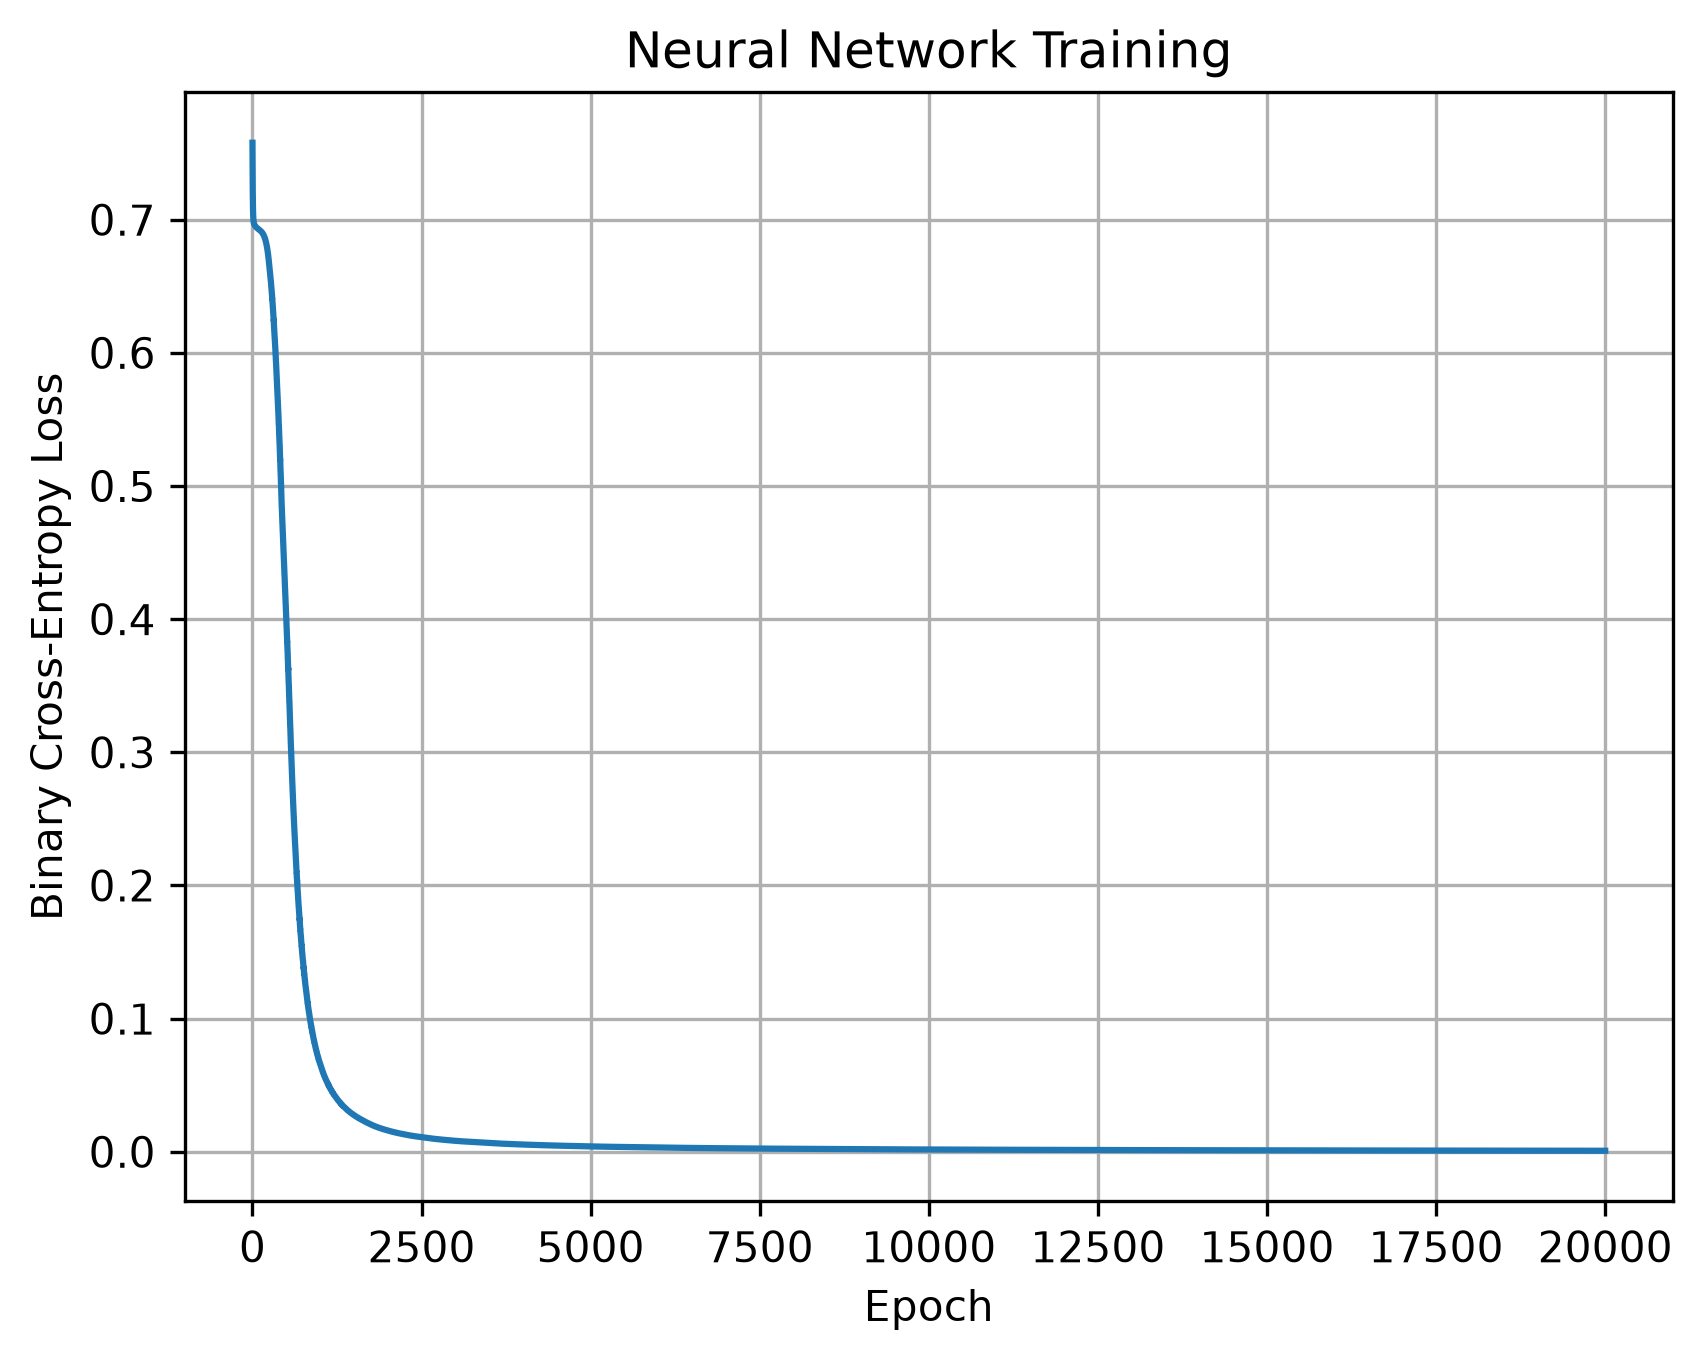
\includegraphics[width=0.82\textwidth]{training_loss.png}
}{
    \fbox{\parbox{0.82\textwidth}{\centering
    Gráfico no encontrado. Ejecutar \texttt{main.py} con el guardado de figura habilitado y colocar \texttt{training\_loss.png} junto a este informe.}}
}
\caption{Evolución de la pérdida durante el entrenamiento.}
\end{figure}

Las cuatro predicciones coinciden con las etiquetas del conjunto de entrenamiento. Esto demuestra que la red aprendió a representar los cuatro casos presentados, pero no constituye una evaluación de generalización, ya que no se utilizó un conjunto de prueba independiente.

\section{Conclusiones}
Se implementó y entrenó una red neuronal multicapa utilizando Python y NumPy, programando explícitamente la propagación hacia adelante, la función de pérdida, la retropropagación y la actualización de parámetros. El modelo clasificó correctamente los cuatro ejemplos del problema XOR. La experiencia permitió aplicar los componentes fundamentales del aprendizaje supervisado. Como limitación, el conjunto de datos es mínimo y coincide con los ejemplos de entrenamiento; por ello, los resultados no permiten afirmar capacidad de generalización a datos nuevos.

\section*{Material complementario}
El código fuente y las pruebas se encuentran en el directorio \texttt{Red\_Neuronal}. Para ejecutar el experimento desde la raíz del repositorio:

\begin{verbatim}
python Red_Neuronal/src/main.py
python -m unittest discover -s Red_Neuronal/tests -v
\end{verbatim}

\end{document}